\def\problemset#1#2#3{
\noindent\rule{16.5cm}{1pt}
\begin{center}
  \parbox{16.5cm}{\bf
    STAT 598Z Homework 2 \\
    Instructor: Prof. S V N Vishwanathan \hfill Jiajie Huang\\
    Due Feb 12th, 2013 \hfill huang147@purdue.edu
    }
\end{center}
\noindent\rule{16.5cm}{0.5pt}
}

\newcommand{\lb}[1]{\left \lfloor #1 \right \rfloor}
\newcommand{\bmat}[1]{\begin{bmatrix} #1 \end{bmatrix}}
\documentclass[fleqn, 11pt]{article}
\usepackage{fullpage}
\usepackage{hyperref}
\usepackage{ulem}
\usepackage{amsmath}
\usepackage{algorithm}
%\usepackage{algorithmic}
\usepackage{algpseudocode}
\setlength{\parindent}{0in}
\usepackage{graphics}
\usepackage{graphicx}
\usepackage{mathtools}



\begin{document}

\problemset{3}{Problem Set 2}{\today}


\section*{Problem 1}
\begin{itemize}
\item Create a list x \\\\
Code: 
\begin{verbatim}
x = [9, 10, 11, 12, 13, 14, 15, 16]
print x
\end{verbatim}
Output: 
\begin{verbatim}
[9, 10, 11, 12, 13, 14, 15, 16]
\end{verbatim}


\item Print the last 3 elements of x \\\\
Code: 
\begin{verbatim}
print x[-3], x[-2], x[-1]
\end{verbatim}
Output: 
\begin{verbatim}
14 15 16
\end{verbatim}

\item Print all the even numbers in x \\\\
Code: 
\begin{verbatim}
for num in x:
    if num%2 == 0:
        print num
\end{verbatim}
Output: 
\begin{verbatim}
10
12
14
16
\end{verbatim}

\item Delete all the even numbers in x and print the resulting list \\\\
Code: 
\begin{verbatim}
for i, num in enumerate(x):
    if num%2 == 0:
        x.pop(i)
print x
\end{verbatim}
Output: 
\begin{verbatim}
[9, 11, 13, 15]
\end{verbatim}

\item Create a tuple y from x \\\\ 
Code: 
\begin{verbatim}
y = tuple(x)
print y
\end{verbatim}
Output: 
\begin{verbatim}
(9, 11, 13, 15)
\end{verbatim}

The elements in y are not editable. I tried to insert or delete elements from y:
\begin{verbatim}
y.append(100)
y.pop(9)
\end{verbatim}

Then Python returns with error:
\begin{verbatim}
  File "hw2p1.py", line 26, in <module>
    y.append(100)
AttributeError: 'tuple' object has no attribute 'append'

  File "hw2p1.py", line 27, in <module>
    y.pop(9)
AttributeError: 'tuple' object has no attribute 'pop'
\end{verbatim}

\end{itemize}

\section*{Problem 2}
For this question, I assume that n is a positive integer ($n \geq 1$). Below are the 3 methods calculating $\sum_i^n (1/2)^i$:

\begin{itemize}

\item Getting the sum using a for loop
\begin{verbatim}
while 1:

        n = input("Please input an integer n (n>=1):")

        if n >= 1 and isinstance(n, int) == 1:
                
                sum1 = 0
                for i in range(1, n+1):
                        sum1 += 0.5**i
                print "(for loop) sum is", sum1

                break

        else:
                print "Invalid input! Positive integer required!"
\end{verbatim}


\item Getting the sum using a while loop 
\begin{verbatim}
while 1:

        n = input("Please input an integer n (n>=1):")

        if n >= 1 and isinstance(n, int) == 1:

                # get the sum using a while loop
                sum2 = 0
                i = 1
                while i <= n:
                        sum2 += 0.5**i
                        i=i+1
                print "(while loop) sum is", sum2

                break

        else:
                print "Invalid input! Positive integer required!"
\end{verbatim}



\item Getting the sum without using a loop, but using a summing equation for the geometric series 
\begin{verbatim}
while 1:

        n = input("Please input an integer n (n>=1):")

        if n >= 1 and isinstance(n, int) == 1:

                # get the sum without a loop
                # use the summing equation of geometric series
                sum3 = 1 - 0.5**n
                print "(w/o loop) sum is", sum3

                break

        else:
                print "Invalid input! Positive integer required!"
\end{verbatim}

\end{itemize}

I tried different $n$'s, when $n$ is small ($n < 1000000$), all the three python programs give the same result. 
\begin{verbatim}
Please input an integer n (n>=1):1
(for loop) sum is 0.5
Please input an integer n (n>=1):2
(for loop) sum is 0.75
Please input an integer n (n>=1):3
(for loop) sum is 0.875
Please input an integer n (n>=1):10
(for loop) sum is 0.9990234375
Please input an integer n (n>=1):50
(for loop) sum is 1.0
Please input an integer n (n>=1):1000000
(for loop) sum is 1.0
...

Please input an integer n (n>=1):1
(while loop) sum is 0.5
Please input an integer n (n>=1):2
(while loop) sum is 0.75
Please input an integer n (n>=1):3
(while loop) sum is 0.875
Please input an integer n (n>=1):10
(while loop) sum is 0.9990234375
Please input an integer n (n>=1):50
(while loop) sum is 1.0
Please input an integer n (n>=1):1000000
(while loop) sum is 1.0
...

Please input an integer n (n>=1):1
(w/o loop) sum is 0.5
Please input an integer n (n>=1):2
(w/o loop) sum is 0.75
Please input an integer n (n>=1):3
(w/o loop) sum is 0.875
Please input an integer n (n>=1):10
(w/o loop) sum is 0.9990234375
Please input an integer n (n>=1):50
(w/o loop) sum is 1.0
Please input an integer n (n>=1):1000000
(w/o loop) sum is 1.0
...
\end{verbatim}


When $n = 1$, $sum = 0.5$; when $n = 2$, $sum = 0.75$; when $n = 3$, $sum = 0.875$; ... ; when $n = 10$, $n = 0.9990234375$; ... ; when $n = 50$, $n$ has become so close to 1 that the result is printed out as $sum = 1.0$ on the screen. When $n$ is very large, $sum$ asymptotically equals $1$, but the amount of steps needed to calculate loops gets significantly huge. I tried $n = 10000000000000$, the program using for loop and while loop got into memory problem and crashed; but the program using no loop still worked as normal and returned the result within $1$ sec. Here I'm showing the error message returned by the for loop as example: 

\begin{verbatim}
Traceback (most recent call last):
  File "hw2p2_forloop.py", line 8, in <module>
    for i in range(1, n+1):
MemoryError
\end{verbatim}

The reason for the memory error in the for loop here is, using $range(1, n + 1)$ is creating an array that contains numbers from $1$ to $n + 1$, when $n$ gets large, it exhausts the memory and returns an error. \\ 

I also analyzed the computational complexity of the 3 programs:
\begin{itemize}
\item For loop: $\Theta(n)$ (both $O(n)$ and $\Omega(n)$), takes $n$ steps to get the sum
\item While loop: $\Theta(n)$ (both $O(n)$ and $\Omega(n)$), takes $n$ steps to get the sum
\item No loop: $\Theta(1)$ (both $O(1)$ and $\Omega(1)$), only takes $1$ step to get the sum 
\end{itemize}

Therefore, when $n$ gets huge, for loop and while loop take huge amount of steps to get done, but summing formula still only takes 1 step. \\

To make the program more robust to errors when $n$ is large in for loops, we can modify the code from using $range$ to using $xrange$. The advantage of using $xrange$ is that, it always takes the same amount of memory despite of the size of the range, so it won't exhaust the memory even when $n$ is large.    Code shown below: 

\begin{verbatim}
while 1:

        n = input("Please input an integer n (n>=1):")

        if n >= 1 and isinstance(n, int) == 1:
                
                sum1 = 0
                for i in xrange(1, n+1):
                        sum1 += 0.5**i
                print "(for loop) sum is", sum1

                break

        else:
                print "Invalid input! Positive integer required!"
\end{verbatim}

Another way is to try to take the algorithm of lower computational complexity, which requires less basic operational steps to finish. \\



\section*{Problem 3}
\begin{itemize}
\item $x^3$ is $O(x^3)$ and $\Theta (x^3)$ but not $\Theta (x^4)$. Prove:\\\\
If $x^3 = O(x^3)$, then we have 
\[
0 \leq x^3 \leq cx^3
\]
Divide $x^3$ at both sides, then 
\[
0 \leq 1 \leq c
\]
Thus $c = 1$, and any $x \geq x_0 = 1$ will satisfy 
\[
0 \leq x^3 \leq 1 \cdot x^3 = x^3
\]
$x^3 = O(x^3)$ proved. 

For $x^3 = \Theta(x^3)$, we know 
\[
\lim_{x->\infty} \frac{x^3}{x^3} = 1 > 0 
\]
But 
\[
\lim_{x->\infty} \frac{x^3}{x^4} = 0 
\]
So $x^3 \neq \Theta(x^4)$. \\\\
Therefore, in conclusion, $x^3$ is $O(x^3)$ and $\Theta (x^3)$ but not $\Theta (x^4)$. Proved. \\

\item $(n + a)^b = \Theta(n^b)$. Prove:\\\\
By binomial series we have 
\[
(n + a)^b = n^b + C_b^1n^{b-1}a + C_b^2n^{b-2}a^2 + ... + C_b^{b-1}na^{b-1} + a^b 
\]
Thus 
\[
\lim_{n->\infty} \frac{(n + a)^b}{n^b} 
= \frac{n^b + C_b^1n^{b-1}a + C_b^2n^{b-2}a^2 + ... + C_b^{b-1}na^{b-1} + a^b }{n^b} 
\]
\[= 1 + \frac{C_b^1a}{n} + \frac{C_b^2a^2}{n^2} + ... + \frac{C_b^{b-1}a^{b-1}}{n^{b-1}} + \frac{a^b}{n^b} 
= 1 > 0
\]
By definition we have $(n + a)^b = \Theta(n^b)$. Proved. \\


\item $(\log(n))^k = O(n)$. Prove:\\\\
We need to prove $0 \leq (\log(n))^k \leq cn$, where $c$ is a constant. As we already know that $n$ is a positive integer, so $0 \leq (\log(n))^k$ is always true, no matter what $k$ is. \\\\
For the $(\log(n))^k \leq cn$ part, if $k \leq 0$, when $n$ gets large, $(\log(n))^k$ becomes a small number, $(\log(n))^k \leq cn$ also holds. If $k > 0$, we need to prove that there exists a $c$, so that $c \geq \frac{(\log(n))^k}{n}$ when $n->\inf$. And we know exponential growth dominates polynomial growth, so $n$ will dominate $(\log(n))^k$ when $n$ is large, thus we are able to get a constant $c$ that satisfies $c \geq \frac{(\log(n))^k}{n}$. Proved. \\



\item $\frac{n}{n + 1} = 1 + O(\frac{1}{n})$. Prove: \\\\
For any $n$ as a positive integer, we have 
\[
0 \leq \frac{n}{n + 1} \leq \frac{n + 1}{n + 1} \leq \frac{n + 1}{n} \leq \frac{n + 2}{n} \leq ... \leq \frac{n + c}{n} = 1 + c(\frac{1}{n})
\]
By definition we have $\frac{n}{n + 1} = \Theta (\frac{1}{n})$. Proved. \\







\item $\sum_{i = 0}^{\log_2(n)} 2^i = \Theta(n)$. Prove:\\\\
In this problem, we assume that $\log_2(n)$ is an integer; in other words, if it is not an integer, the summation only sums up to the nearest integer below $\log_2 (n)$, which is
\[
\sum_{i = 0}^{\log_2(n)} 2^i = 2^0 + 2^1 + ... + 2^{\log_2(n)} \]
\[
= 2^0 \frac{2^{\log_2(n)} - 1}{2 - 1} = 2^{\log_2(n)} - 1 = n - 1
\] 
And we know 
\[
\lim_{n->\infty}\frac{n-1}{n} = 1 > 0
\]
So $n - 1 = \Theta(n)$, which is equivalent to $\sum_{i = 0}^{\log_2(n)} 2^i = \Theta(n) $. Proved. \\

\end{itemize}

\section*{Problem 4}
\begin{itemize}
\item This is a recursive function. It is computing $mystery(x, n) = x^n$. At each step, this function evaluates $n$, if $n = 0$, return $mystery(x, n) = 1$; else if $n$ is an odd number, return $mystery(x, n-1)*x$; or if $n$ is an even number, return $[mystery(x, n/2)]^2$. 


\item The complexity of this algorithm depends on two aspects: 
\begin{itemize}
\item The number of basic operations at each step. For this function, at each step, the number of basic operations is only $1$ (either $mystery(x, n-1)*x$ or $[mystery(x, n/2)]^2$, one multiplication only at each step). 
\item The number of total steps. Starting as $n$, the speed of $n$ to get smaller is different depending on whether it is odd or even. If we are lucky, $n$ is the exponential of $2$, in other words, $n = 2^k$ (k is a positive integer), then $n$ gets to $n/2$ for the next step, then $n/2^2$ next, ..., until it gets to $1$. That is the best case for this algorithm while the number of steps is minimal. However, for the worst case, $n$ would be an odd number, the next step we only take $n-1$, and then $\frac{n-1}{2}$ next, then if $\frac{n-1}{2}$ is an odd number again, we need to take $\frac{n-1}{2}-1$, then $\frac{\frac{n-1}{2}-1}{2}$... So in worst case, the recursion tree is shown in Figure \ref{recursion} below: 

\begin{figure}[htb]
\centering
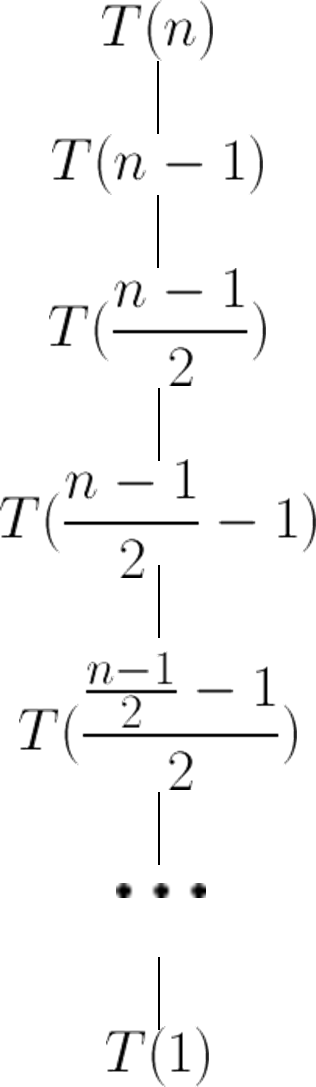
\includegraphics[width=2cm]{p4.png}
\caption{Recursion Tree for $mystery(x,n)$}
\label{recursion}
\end{figure}

\end{itemize}

Then the time complexity of worst case (given $n$ is odd) 
\[T(n) = T(n-1) + 1 \]
\[= T(\frac{n-1}{2}) + 1 + 1 \]
\[= T(\frac{n-1}{2}-1) + 1 + 1 + 1\] 
\[= T(\frac{\frac{n-1}{2}-1}{2}) + 1 + 1 + 1 + 1 \]
\[= ... = T(1) + m \] 
Or to make it clear
\[T(n) = T(n-1) + 1 = T(\frac{n-1}{2}) + 2 = T(\frac{n-1}{2}-1) + 3 = \frac{\frac{n-1}{2}-1}{2} + 4 = ... = T(1) + m 
\]

The $+1$ in each step is the basic operation taken in each step; $m$ is the number of total steps. We can easily see that in the worst case, we have odd and even indices alternatively, which means for $m/2$ steps we are only subtracting the current index by $1$, and for another $m/2$ steps we are dividing the current index by $2$, to get the index of next step. Thus in the last step, $T(\frac{n}{2^{\frac{m}{2}}}) = T(1)$, so $\frac{n}{2^{\frac{m}{2}}} = 1$, we get $m = 2\log_2(n)$. So the total complexity is 
\[
T(n) = T(1) + m = T(1) + 2\log_2(n) = O(2\log_2(n))
\]
And the big-O complexity for the worst case is the one for the whole algorithm. So the total complexity for the algorithm is $O(2\log_2(n))$\footnote{Note: I talked to Nick Fico for a few questions on this homework. }.

\end{itemize}


\end{document}